%%%%%%%%%%%%%%%%%%%%%%%%%%%%%%%%%%%%%%%%%%%%%%%%%%%%
%%%                                              %%%
%%%     Language Science Press Master File       %%%
%%%         follow the instructions below        %%%
%%%                                              %%%
%%%%%%%%%%%%%%%%%%%%%%%%%%%%%%%%%%%%%%%%%%%%%%%%%%%%
 
% Everything following a % is ignored
% Some lines start with %. Remove the % to include them

\documentclass[output=short             % long|short|inprep              
% 	        ,blackandwhite
% 		,smallfont
  	        ,draftmode  
		,biblatex
		  ]{LSP/langsci}    
  
%%%%%%%%%%%%%%%%%%%%%%%%%%%%%%%%%%%%%%%%%%%%%%%%%%%%
%%%                                              %%%
%%%          additional packages                 %%%
%%%                                              %%%
%%%%%%%%%%%%%%%%%%%%%%%%%%%%%%%%%%%%%%%%%%%%%%%%%%%%

% put all additional commands you need in the 
% following files. If you do not know what this might 
% mean, you can safely ignore this section

%%%%%%%%%%%%%%%%%%%%%%%%%%%%%%%%%%%%%%%%%%%%%%%%%%%%
%%%                                              %%%
%%%                 Metadata                     %%%
%%%          fill in as appropriate              %%%
%%%                                              %%%
%%%%%%%%%%%%%%%%%%%%%%%%%%%%%%%%%%%%%%%%%%%%%%%%%%%%

% \subtitle{}
% \BackTitle{} % Change if BackTitle != Title
\BackBody{}
%\dedication{Change dedication in localmetadata.tex}
%\typesetter{Change typesetter in localmetadata.tex}
%\proofreader{Change proofreaders in localmetadata.tex}
\author{ocket88888}

\renewcommand{\lsISBN}{978-0-000000-00-0}                     
\renewcommand{\lsSeries}{bbos} % use lowercase acronym, e.g. sidl, eotms, tgdi
\renewcommand{\lsSeriesNumber}{99} %will be assigned when the book enters the proofreading stage
\renewcommand{\lsURL}{http://langsci-press.org/catalog/book/00} % contact the coordinator for the right number

% add all extra packages you need to load to this file  
\usepackage{tabularx} 

%%%%%%%%%%%%%%%%%%%%%%%%%%%%%%%%%%%%%%%%%%%%%%%%%%%%
%%%                                              %%%
%%%           Examples                           %%%
%%%                                              %%%
%%%%%%%%%%%%%%%%%%%%%%%%%%%%%%%%%%%%%%%%%%%%%%%%%%%% 
\usepackage{./LSP/lsp-styles/lsp-gb4e} 
%% to add additional information to the right of examples, uncomment the following line
% \usepackage{jambox}
%% if you want the source line of examples to be in italics, uncomment the following line
% \renewcommand{\exfont}{\itshape}
%% hyphenation points for line breaks
%% Normally, automatic hyphenation in LaTeX is very good
%% If a word is mis-hyphenated, add it to this file
%%
%% add information to TeX file before \begin{document} with:
%% %% hyphenation points for line breaks
%% Normally, automatic hyphenation in LaTeX is very good
%% If a word is mis-hyphenated, add it to this file
%%
%% add information to TeX file before \begin{document} with:
%% %% hyphenation points for line breaks
%% Normally, automatic hyphenation in LaTeX is very good
%% If a word is mis-hyphenated, add it to this file
%%
%% add information to TeX file before \begin{document} with:
%% \include{localhyphenation}
\hyphenation{
affri-ca-te
affri-ca-tes
com-ple-ments
}
\hyphenation{
affri-ca-te
affri-ca-tes
com-ple-ments
}
\hyphenation{
affri-ca-te
affri-ca-tes
com-ple-ments
}
%add all your local new commands to this file
%%%%%%%%%%%%%%%%%%%%%%%%%%%%%%%%%%%%%%%%%%%
%%%                                     %%%
%%%      Language Syntax Definitions    %%%
%%%                                     %%%
%%%                                     %%%
%%%%%%%%%%%%%%%%%%%%%%%%%%%%%%%%%%%%%%%%%%%
\definecolor{codeBlue}{rgb}{0,0.8,0.1}
\definecolor{codeGreen}{rgb}{0,0.1,0.8}
\definecolor{codePurple}{rgb}{0.58,0,0.82}
\definecolor{codeGray}{rgb}{0.5,0.5,0.5}
\definecolor{backcolor}{rgb}{0.95,0.95,0.92}


%BrenMat (for Maths)
\lstdefinestyle{BrenMat}{
backgroundcolor=\color{backcolor},
commentstyle=\color{codeGray},
keywordstyle=\color{codeBlue},
stringstyle=\color{codePurple},
numberstyle=\tiny\color{codeGreen},
basicstyle=\footnotesize,
breakatwhitespace=false,
breaklines=true,
captionpos=b,
keepspaces=true,
numbers=left,
numbersep=5pt,
showspaces=false,
showstringspaces=false
showtabs=false,
tabsize=2
}
\newcommand{\smiley}{:)} 
\bibliography{localbibliography} 

%%%%%%%%%%%%%%%%%%%%%%%%%%%%%%%%%%%%%%%%%%%%%%%%%%%%
%%%                                              %%%
%%%             Frontmatter                      %%%
%%%                                              %%%
%%%%%%%%%%%%%%%%%%%%%%%%%%%%%%%%%%%%%%%%%%%%%%%%%%%%
\begin{document}              
\maketitle                
\frontmatter
% %% uncomment if you have preface and/or acknowledgements

\tableofcontents
% \addchap{Preface}
\begin{refsection}

%content goes here

\printbibliography[heading=subbibliography]
\end{refsection}
% \addchap{Acknowledgments}
\begin{refsection}

%content goes here

\printbibliography[heading=subbibliography]
\end{refsection}
% \addchap{List of abbreviations}
\begin{refsection}

%content goes here

\printbibliography[heading=subbibliography]
\end{refsection} 

\mainmatter         
 

%%%%%%%%%%%%%%%%%%%%%%%%%%%%%%%%%%%%%%%%%%%%%%%%%%%%
%%%                                              %%%
%%%             Chapters                         %%%
%%%                                              %%%
%%%%%%%%%%%%%%%%%%%%%%%%%%%%%%%%%%%%%%%%%%%%%%%%%%%%

\chapter{Building Blocks: Basic Data Types}
\lstset{style=BrenMat}

Add content in chapters/01.tex.

\section{Functions}

Functions are incredibly useful constructs throughout mathematics, the natural sciences, and in particular
computer science. Functions take any number of inputs, or arguments, usually performing operations on those arguments to
produce an output. The definition of a function takes the following form:
\begin{center}
\begin{lstlisting}[language=C,caption=Function Example,label=lst:funcEx]
type FunctionName[type ArgumentName0, type ArgumentName1, ... type ArgumentNameN]{
	Operations;
	return Possible Output;
}
\end{lstlisting}
\end{center}

As seen above, the first word is "type," which refers to the type of data that the result, or output, of the function will be. In later chapters we will define more of these data-types, but for now we'll introduce the most simple.
"void" is the type of data that doesn't exist. That is to say, a function of type void not produce a result, and is typically used only to modify the arguments.
It should be noted that an argument cannot be of this type, as it's kind of nonsensical to pass no information as an argument. \\
The second word is "FunctionName," which is, perhaps obviously, a placeholder for the name of the function. A reader with any amount of experience with trigonometry will recognize the function name Sine, for example. When using a function, only the name of and arguments to the function need be provided for its use to be complete and valid. \\
After the function name, a list of comma-separated arguments, with their own types, are specified. A function may take any number of arguments, but the most common is simply one. In cases of multiple arguments the order of the arguments is important. A datum of type A may not be passed to a function that only accepts one argument of type B. Similarly, a function that takes one argument of type A, and then an argument of type B cannot be used on one argument of type B, and then an argument of type A. \\
The placeholders "Operations" and "Possibly Output" are contained within curly braces (\{ and \}). This serves to make entirely explicit the operations that the function performs, so that they may not be confused with any work done directly above or beneath them. \\
"return" is used to specify that what follows is the output of the function. Traditionally, this is also the endpoint of the function. That is, any operations after it are ignored. For this reason, even functions that have the "void" type may return nothing to indicate that computation is to cease at that point, but it is certainly not required. \\
Lastly, the end of every line within the function definition ends with a semicolon. The semicolon serves to indicate the end of one operation, and is used rather than just a new line because sometimes a mathematician may choose to write multiple operations on one line due to space constraints or personal styling preference. \\
Functions are used in a similar manner to this throughout many computer science languages. Specifically, those familiar with Java or C may find 
\ref{lst:funcEx} to be reminiscent of those languages. Please note that the above is NOT representative of any programming language, it is merely a way of organizing definitions of mathematical operations. \\
The way a function is used is called "calling" that function, and it takes the following form:
\begin{center}
\begin{lstlisting}[language=C, caption=Function Call Example, label=lst:funcCallEx]
FunctionName[ArgumentName0, ArgumentName1, ... ArgumentNameN]
\end{lstlisting}
\end{center}
The first word this time is "FunctionName," which differs from \ref{lst:funcEx} in that it does not specify a type. Since you cannot use a function that does not exist, the type of the function's result has already been set, and does not need to be specified again. \\
This function call also differs from \ref{lst:funcEx} in that it's arguments are not typed. Just as the function type need not be respecified, the type of the arguments has already been decided, and the burden of remembering which arguments are what type rests on the shoulders of the person writing the function call.

\section{Integers}
At this point it will be useful to define a data type that is not simply "void". Many readers will already be familiar with the concept of integers, but this chapter exists largely for the purpose of rigorously defining perhaps somewhat simple ideas. \\


\subsection{Whole Numbers and the Successor Function}
Our starting point isn't to begin defining the integer, but to describe a new data type, the "whole number," which will be abbreviated in writing mathematical expressions as "wn". The definition begins with one member from which all others are defined. That is to say:
\begin{center}
\textit{$0$ is the first whole number}
\end{center}

Don't worry about the definition of $0$'s value right now, that will become apparent shortly. \\
Every other whole number can be obtained from a recursive definition using the so-called "Successor Function" in the following way:
\begin{center}
\begin{lstlisting}[language=C, caption=Successor Function,label=lst:sucFunc]
wn SuccessorFunction[wn n]{
	return the next successive whole number
}
\end{lstlisting}
\end{center} 
This can also be expressed in the following way:
\begin{center}
$SuccessorFunction[0] = 1$\\
$SuccessorFunction[1] = 2$\\
Successor Function Example\label{eq:sucFuncEx}
\end{center}
This implies that the numbers $0$-$9$ are just symbols attributed to the whole numbers generated by by the Successor Function. It is commonplace to use what is known as a "base-ten number system," which means that upon reaching 9, two characters arise to take its place, starting with a $1$ in the furthest left, and a $0$ on the right. The place a number holds is called its digit. In general, whenever a digit reaches 9, the digit directly to the left has the Successor Function called on it, which increments the digit. If there is no digit to the left, it is treated as $0$, which produces the whole number $1$ in that digit. Keep in mind that this is simply a way of representing an infinite number of outputs of the Successor Function, and as such should be thought of collectively as one whole number, not a collection of whole numbers. \\


\subsection{Addition}

It is easy to see at this point how simple arithmetic operations can be defined. The difference between operations and functions is largely immaterial, in fact it is useful to define operations as functions first, then show the symbol. For instance, addition can be described in the following way:
\begin{center}
\begin{lstlisting}[language=C,caption=Addition Function,label=lst:addFunc]
wn PlusOne[wn x]{
	return SuccessorFunction[x];
}
\end{lstlisting}
Output: $x+1$
\end{center}
So as seen above, adding one to a number is the same as calling the Successor Function on it (which may have been obvious by now). Then adding a number greater than one to some whole number 'x' is as simple as calling the successor function that many times. We can now easily define a symbol '+' to represent calling the successor function x times on a whole number y if given in the form $x+y$. At this point it is useful to note that
\begin{center}
$SuccessorFunction[2]=3=SuccessorFunction[SuccessorFunction[1]]$
\end{center}
which is a simple way of saying that $2+1=1+2$, known as the associative property of addition. \\
It is here that the value of $0$ becomes apparent. For example, consider the statement $1+0$. We know from above that this is equivalent to the statement $SuccessorFunction[0]=1$. From here it is trivial to show that any whole number that has the number $0$ added to it retains its value.

\subsection{Negative Numbers and Subtraction}
Before going any further, we will develop our understanding of whole numbers into an understanding of integers. Like with whole numbers, the easiest place to start is with a function.
\begin{center}
\begin{lstlisting}[language=C,caption=The Predecessor Function,label=lst:predFunc]
wn PredecessorFunction[wn x]{
	Find a number y such that SuccessorFunction[y]=x;
	return y;
}
\end{lstlisting}
\end{center}
The Predecessor Function, it would seem, only undoes the Successor Function, and as such is sometimes called the Inverse Successor Function. Like with addition, it may be useful to think of the operation of subtraction as an implementation of this function.
\begin{center}
\begin{lstlisting}[language=C,caption=Minus One Function,label=lst:minusOneFunc]
wn MinusOne[wn x]{
	return PredecessorFunction[x];
}
\end{lstlisting}
\end{center}
The above function can be used to describe $x-1$, and in general subtraction of a whole number x from a whole number y is defined as calling the Predecessor Function x times on y, given the form $y-x$. \\
It is now easy to define all negative numbers as simply a number for which the operations of the Successor Function and the Predecessor Function are switched. That is to say that for a number x and a number y, $y+x=y- Negative x$. There exists then a number z for every y such that $y+z=0$, which means that when adding the negative number z to y, the Predecessor Function is called on y exactly as many times as the Successor Function must be called on $0$ to obtain the value y. This is the definition of Negative y, meaning $z=Negative y$ \\
Because whole numbers obey the original definitions of addition and subtraction, these new negative numbers cannot be said to be whole numbers. The name of these new numbers, in conjunction with the whole numbers, is "integers" (abbreviated "int" in mathematical expressions). \\
It is implied, of course, that this means that calling the Predecessor Function x times on $0$ produces Negative x, that is to say that $0-1=Negative 1$. Furthermore, because writing out "Negative" every time subtraction is used can get a bit cumbersome and cluttered, and because of their unique property that adding is subtracting and subtracting is adding, negative numbers are written in the notation
\begin{center}
$Negative x = -x$
\end{center}
This is because there is an implicit $0$ to the left of the $-x$, which is omitted simply because that too would get repetitive, and only the symbol '$-$' is required to indicate the negativity of an integer x. For integers, it can be seen that the statement $x-y$ is equivalent to the statement $x+Negative y = x+ -y$

\section{Sets}
A set isn't so much a data-type as a way of organizing data. Sets are useful throughout all fields of natural sciences, computer science, math and logic as a way of describing large (sometimes infinite) amounts of data. A set contains only information on the unique objects it contains, and not any information about the ordering thereof. For example, suppose I have a set A that initially contains nothing, which incidentally has its own symbol: $\varnothing$.
\begin{center}
\begin{figure}[h]
\caption{Set A} \label{fig:setAEmpty}
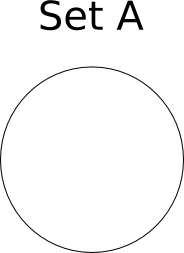
\includegraphics[scale=0.5]{figures/setAEmpty.png}
\end{figure}
\end{center}

Now suppose I add the integer $1$ to set A.
\begin{center}
\begin{figure}[h]
\caption{Set A} \label{fig:setA1}
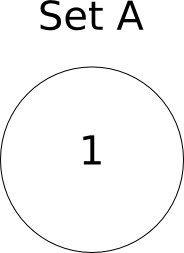
\includegraphics[scale=0.5]{figures/setA1.png}
\end{figure}
\end{center}

If I were to try to add $1$ to set A again, this is what set A would look after I attempt that operation:

\begin{center}
\begin{figure}
\caption{Set A} \label{fig:setA1_0}
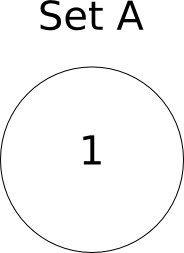
\includegraphics[scale=0.5]{figures/setA1.png}
\end{figure}
\end{center}

See, the set remains unchanged upon adding an element that it already contains. \emph{A set only contains information about the \textbf{unique} items it contains}. \\
Now suppose that I added the integer $2$ to this set.

\begin{center}
\begin{figure}
\caption{SetA} \label{fig:setA12}
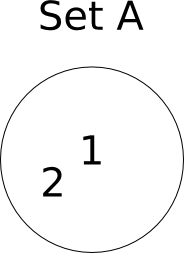
\includegraphics[scale=0.5]{figures/setA12.png}
\end{figure}
\end{center}

As seen above, there is no notion of the order or rank of the elements of A. Even though $1$ was added to the set before $2$, $1$ holds no special position, and the two integers are treated equally. There is a special, named set for the set that contains all whole numbers, denoted '$\mathbb{W}$', and the set that contains all integers, commonly denoted '$\mathbb{Z}$'.

\section{Multiplication and Division}
Before we can continue to build up sets of useful constructs, we first need to define some more operations that can be preformed on integers (specifically division will be of interest later). \\

\subsection{Multiplication}
Of the two operations that make up the title of this section, multiplication is the easier of the two to explain. The following function describes it in loose terms.
\begin{center}
\begin{lstlisting}[language=C,caption=Multiplication Function,label=lst:multFunc]
int Multiply[int x, int y]{
	int result = x_1 + x_2 + x_3 ... + x_y;
	return result;
}
\end{lstlisting}
\end{center}

What this means, in English, is that multiplying x by y returns x added to x y times. For this reason, expressions of the form $x\times y$ are typically pronounced "x times y", and the '$\times$' symbol denotes multiplying the left side by the right side. This is often abbreviated, as the $\times$ symbol can be confused with a variable named x, as simply $xy$. This is syntactically unambiguous because all variable and function names require formatting called 'Camel Case' which means that the first letter of the name of the variable or function may be lowercase, but every time another word is added, its first letter must be capitalized. For example, 'thisIsAVariable' is a valid variable name, but 'thisisambiguous' is not. However, because it is common for function and variable names to only be one word long, the $\times$ symbol is often used to delimit them (e.g. $a\times var$).


\subsection{Division}
To put it as simply as possible, division is the operation that undoes multiplication. However, similar to subtraction, order matters. For instance, if z is the output of $x\times y$, then the output of dividing z by x is y. Similarly, the output of z divided by y is x. Because order matters, dividing y by z is \emph{not} the same as dividing z by y. Here is a loosely-written function that helps to describe that process.
\begin{center}
\begin{lstlisting}[language=C,caption=Division Function,label=lst:divFunc]
int DivideBy[int x, int y]{
	return the integer y is multiplied by to obtain x;
}
\end{lstlisting}
\end{center}
There are, however, many cases where there is no integer that y can be multiplied by to obtain x. Consider, for example, the division of $5$ by $3$ (there is no integer y such that y times 3 outputs 5). In these cases, the output is left in the form of what is known as a 'fraction'. Fractions take the form $\frac{x}{y}$ or $x/y$ when dividing x by y. The difference between them is accounted for by the versatility of the environment in which it is written, $\frac{x}{y}$ is the preferred form, but $x/y$ may be used when such typesetting is unavailable. To provide consistency with a planned programming language, the form $x/y$ will be used because text editors only support this form. \\
In a base ten number system, it becomes bothersome to always write fractions this way, but to understand it we must first describe some properties of fractions. \\
The value of a fraction is invariant under multiplication of both the top (called the 'numerator') and the bottom (called the 'denominator') by the same integer. Because division is merely the inverse of multiplication, the same must be true for division.
\begin{center}
\begin{equation}
x / y = \frac{x}{y} = \frac{x\times c}{y \times c} = \frac{x / c}{y / c}
\end{equation}
\end{center}
























  %add a percentage sign in front of the line to exclude this chapter from book
\chapter{Formal Syntax and Operators}
This chapter is not really meant to be read from top to bottom, only to be used as a reference when reading later chapters. If the way anything is worded is confusing, this chapter is meant to act as a guide. Certain similarities to computer science may become apparent in the way that mathematical expressions are written, and this is not a coincidence but it cannot be stressed enough that this is \emph{not} a programming language (yet).

\section{Boolean Logic}
A basic datatype not covered in Chapter 1, but is also extremely useful is what's known as a 'boolean,' abbreviated 'bool'. This is much simpler to define than a set of numbers, because rather than infinite possible values, there are only two: true or false. This is useful in cases when operations are to be preformed conditionally, or procedurally. For example, the famous Dirac Delta function models the density of a point-mass and has the following form:
\begin{lstlisting}[language=C,caption=Dirac Delta Function,label=lst:dirdelFunc,mathescape]
real $\delta$[real x]{
	if[x==0]{
		return Infinity;
	}
	else{
		return 0;
	}
}
\end{lstlisting}
The first thing immediately apparent is the use of the new function 'if'. If is a special function that allows preforming of mathematical operations within the curly braces that follow it if and only if the expression inside of its arguments evaluates to true. If only takes one argument, though there is no limit to the size of the logical expression that can be passed. The special argument-less function else contains within its 
\subsection{Boolean Operators}
In order to understand the types of arguments that 'if' can take, we must first define some functions that return bool's. The one used in \ref{lst:dirdelFunc} will be a good place to start.
\begin{lstlisting}[language=C,caption=Equivalence Function,label=lst:equivFunc,mathescape]
bool Equivalent[any x, any y]{
	return true if x is equivalent to y, or false if not;
}
\end{lstlisting}
The symbol '==' is used to denote calling Equivalent[x,y] given the form 'x==y'. This is different than '=' because '=' implies assigning a value, whereas after finding the output of 'x==y' the value of x does not become y, or vice-versa. Note that the type used to pass these arguments is 'any' which predictably means that they may be of any type. This is because it is easy to tell if two things are the same type, and if they are not then they cannot be equivalent, which allows sometimes for very easy evaluation of Equivalent's output. \\
The next two operators are very similar, and likely very familiar.

\chapter{Change title for chapter 3 in chapters/03.tex}
Add content in chapters/03.tex\footnote{\citet{Comrie1981} is still useful for diversity linguistics. \is{diversity linguistics}}
% copy the lines above and adapt as necessary
 

%%%%%%%%%%%%%%%%%%%%%%%%%%%%%%%%%%%%%%%%%%%%%%%%%%%%
%%%                                              %%%
%%%             Backmatter                       %%%
%%%                                              %%%
%%%%%%%%%%%%%%%%%%%%%%%%%%%%%%%%%%%%%%%%%%%%%%%%%%%%

% There is normally no need to change the backmatter section
\backmatter
\phantomsection%this allows hyperlink in ToC to work
\addcontentsline{toc}{chapter}{List of references}
\printbibliography   
   
\addcontentsline{toc}{chapter}{Index} 

\phantomsection 
\addcontentsline{toc}{section}{Name index}
\ohead{Name index} 
\printindex 
  
\phantomsection 
\addcontentsline{toc}{section}{Language index}
\ohead{Language index} 
\printindex[lan] 
  
\phantomsection 
\addcontentsline{toc}{section}{Subject index}
\ohead{Subject index} 
\printindex[sbj]
\end{document} 

% you can create your book by running
% xelatex lsp-skeleton.tex
%
% you can also try a simple 
% make
% on the commandline